\scanpage{4}
\mspage{2}
\margin{\begin{tikzpicture}\draw (0,0)--(.6,-.65);\end{tikzpicture}}

$\ell-8$\quad pourquoi\quad \uline{donc}\qquad ?

\rule{\linewidth}{0.3pt}

p3\quad $\ell-8,-9$\qquad $B$ ?

\rule{\linewidth}{0.3pt}

p4.\quad 1.3.1.\quad As tu vérifié si l'accouplement d'A. \unsure{M|$\Pi$}. coïncide avec le tien ?

$\ell\,4$.\quad \uline{formellement} non ramifié ?

$\ell\,7$.\quad \uline{séparablement} clos ?

$\ell\,14-20$.\quad Est-ce utile à dire, en l'absence de référence à ce que ce peut vouloir dire ?

$\ell-5$\quad Qu'il soit\qquad et\qquad signifierait\qquad plutôt ?

\rule{\linewidth}{0.3pt}

pg5\quad $\ell-2$\quad français :\quad les classes $\unsure{w|\omega}$\qquad \uline{en}\qquad relatifs.

\rule{\linewidth}{0.3pt}

pg6\quad $\ell\,4$\quad français.\quad dire\quad un Module inversible simple\qquad ?

\deleted{\illegible{5}}

\figure{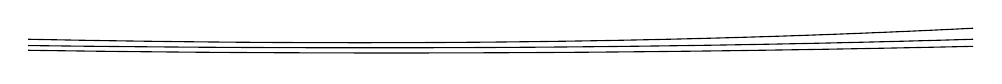
\begin{tikzpicture}\draw (0,.08).. controls (4,0) and (8,.02) .. (12,.22);\draw (0,0).. controls (4,-.05) and (8,-.04) .. (12,.08);\draw (0,-.06).. controls (4,-.12) and (8,-.10) .. (12,-.01);\end{tikzpicture}}

\reversemarginpar
\margin{\textcircled{\textcircled{2}}}
\normalmarginpar
pg7\quad français \uline{$\ell-9$}\quad \begingroup\setbox0=\hbox{$\unsure{\subset|<}$}\hbox{\rlap{\begin{tikzpicture}[overlay,baseline=0pt]\draw[gray,line width=.35pt] (1pt,13pt) .. controls (-7pt,9pt) and (-6pt,-7pt) .. (3pt,-8pt) .. controls (\dimexpr\wd0+10pt\relax,-5pt) and (\dimexpr\wd0+10pt\relax,12pt) .. (\dimexpr\wd0+2pt\relax,14pt) .. controls (6pt,15pt) and (5pt,13pt) .. (4pt,12pt);\end{tikzpicture}}\box0}\endgroup $\unsure{\dot{L}_0|i_0}$\quad donc \textcircled{c'} est

\deleted{$\ell-7$\quad \unsure{si|ni}\quad \illegible{1}\quad que}
\quad $\ell-7$\quad \begingroup\setbox0=\hbox{que}\hbox{\rlap{\begin{tikzpicture}[overlay,baseline=0pt]\draw[gray,line width=.35pt] (1pt,13pt) .. controls (-8pt,11pt) and (-8pt,-7pt) .. (6pt,-8pt) .. controls (\dimexpr\wd0+10pt\relax,-8pt) and (\dimexpr\wd0+11pt\relax,11pt) .. (\dimexpr\wd0-1pt\relax,14pt);\end{tikzpicture}}\box0}\endgroup (le $2^{\underline{\mathrm{e}}}$)

\rule{\linewidth}{0.3pt}

pg8\quad français\quad $\ell\,4$\quad par exemple\quad
$\overset{\text{\inserted{\begingroup\setbox0=\hbox{pour}\hbox{\rlap{\begin{tikzpicture}[overlay,baseline=0pt]\draw[gray,line width=.35pt] (-4pt,6pt) .. controls (-5pt,-6pt) and (\dimexpr\wd0-1pt\relax,-7pt) .. (\dimexpr\wd0+5pt\relax,-1pt) .. controls (\dimexpr\wd0+8pt\relax,10pt) and (\dimexpr\wd0-1pt\relax,13pt) .. (10pt,12pt);\draw[gray,line width=.35pt] (8pt,12pt) .. controls (1pt,14pt) and (-3pt,10pt) .. (-4pt,8pt);\end{tikzpicture}}\box0}\endgroup\,?}}}{\text{\unsure{à|k}}}$\quad $\ldots$

$\ell-7$\quad \uline{le} terme

\rule{\linewidth}{0.3pt}

pg14.\quad L'argument est un peu immoral; si $X$ et $Y$ sont extensions d'une VA par un tore et si $\varphi:X\longrightarrow Y$ est donné, alors $\varphi$ est strictement compatible à la filtration par le poids et $\varphi$ est une isogénie si et seulement si $T_\ell(\varphi)$ en est une.

\rule{\linewidth}{0.3pt}

\mbox{
\begin{tikzpicture}[overlay]\draw (.8,.08) ellipse (1.0 and .6);\end{tikzpicture}pg\deleted{\unsure{19|15|17}}20.}
\quad Rmq 2.6 a)\quad $S$ est-il un trait dans cette remarque ; sait-on assez sur le passage à la limite et Néron ?

\reversemarginpar
\margin{3}
\normalmarginpar
